This first unit has three parts. The first requires you to run a base
scenario with the Wasatch Front travel demand model, and to retrieve some
results from it. The second part is a TRB-related summary assignment. The final
part is a statistical analysis to demonstrate your understanding of linear
regression models.


\section{Running the Wasatch Front Model}
The purpose of this lab is to show you how to run the Wasatch
Front Travel Model and how to look at the model output in various forms. We are
using the Wasatch Front model for several reasons. Principally, your instructor
is reasonably familiar with it from his previous professional experience. 

The purpose of this document is to show you how to run the Wasatch
Front Travel Model and how to look at the model output in various forms. We are
using the Wasatch Front model for several reasons. Principally, your instructor
is reasonably familiar with it from his previous professional experience. 

But beyond this, there are good reasons to use the Wasatch Front model.  First,
the model is much cleaner than others available to this course, which will help
you find scripts and become familiar with the model procedures.  Second, Salt
Lake City is a major metropolitan area with diverse transportation challenges,
and yet is significantly smaller than comparable cities. We can get serious
answers with less computing time than had we chosen Seattle, Atlanta, or another
city.  Finally, the Wasatch Front model uses Citilabs' CUBE travel demand
modeling software, which is also the implementation used in Atlanta.  Knowing
how to operate the Wasatch Front model will shorten the learning curve on the
Atlanta model, should you be employed locally in your career.

The first section of this document explains the model directory in some detail,
and can be used as a reference throughout the course. The second section is a
laboratory activity that will guide you through setting up and executing a model
run.


\subsection{The Model Folders}
We will use model version 7.0 in this course, which was turned over from the
consultant (Resource Systems Group, Inc.) to the MPO (Wasatch Front Regional
Council) in Spring 2011. You will need to download three files from T-Square and
save them to a common directory on your system:
\begin{description}
	\item{\verb#ModelDocumentation.pdf#} This is the report prepared by the
consultants with information on model calibration, data sources, and model
types. We will use it frequently in this class.
	\item{\verb#InputData_V7.zip#} This compression file contains the
socioeconomic data, the highway networks, and the transit line files for all of
the base and horizon year default analyses (20.2 MB, 67.6 MB unzipped).
	\item{\verb#BlankModel_090112.zip#} This compression file contains all of the
scripts necessary to run the model in a given scenario (35 MB, 128 MB
unzipped).
\end{description}



\subsubsection{Input Data Folder}
This folder, shown expanded in Figure \ref{fig:inputsdir} contains all of the
inputs to the model. You'll eventually become intimately familiar with the
contents of this directory, but you should know what's here initially. There can
be some confusion here, because there is also an \verb#_Inputs/# folder in the
model directory. The \verb#InputData_V7/# directory contains all the potential
input files which you may include in an analysis. The \verb#_Inputs/# folder is
where the model looks for input files relevant to the scenario you are running
at the time. This organization scheme is new in version 7, and allows you to run
multiple related scenarios with the same inputs.

The \verb#MasterNet/# folder contains the master highway network,
\verb#MASTER_MMDDYY.net# file. This file contains information on all the links
and nodes in the network, and should never be changed. If your analysis requires
that you edit the highway network (for instance, to change the number of lanes
on a street in a given year), you should make a copy of the \verb#MASTER_X.net#
file and explicitly change its name before you change the file in any
way.\footnote{In case this is not clear, DO NOT CHANGE THE MASTER HIGHWAY
NETWORK! If you must change the network, change a different file with a
different name. It is almost impossible to check if a highway network file has
been changed.} This way, you will always know what the base conditions are as
defined by the MPO. There are a number of backup copies of the master highway
network, should you ignore the above wisdom and need to replace the master. The
files with the \verb$.VPR$ extension contain viewing preferences for the CUBE
viewer.

Inside \verb#SE_Data/# are database files storing the socioeconomic (SE) information
for each zone in the named year. \verb#SE_2020.dbf# contains the households,
income, employment, and population characteristics of all TAZ's in 2020, for
instance.  The numbers in these files are set by the economists working for the
Governor's Office of Planning and Budget working with the MPO, and the files should
not be changed.\footnote{The motivation not to change these numbers is even
stronger than with the highway network. While you may conceivably want to see what
would happen if you build a new interchange, the practice of changing the
results of complicated economic models that you do not understand is
questionable at best.} The set of available \verb#SE_YYYY.dbf# files dictates which
years you can model. While you could conceivably interpolate the data into a
2022 model year, the justifications for doing so are shaky.

\begin{figure}[tp]
	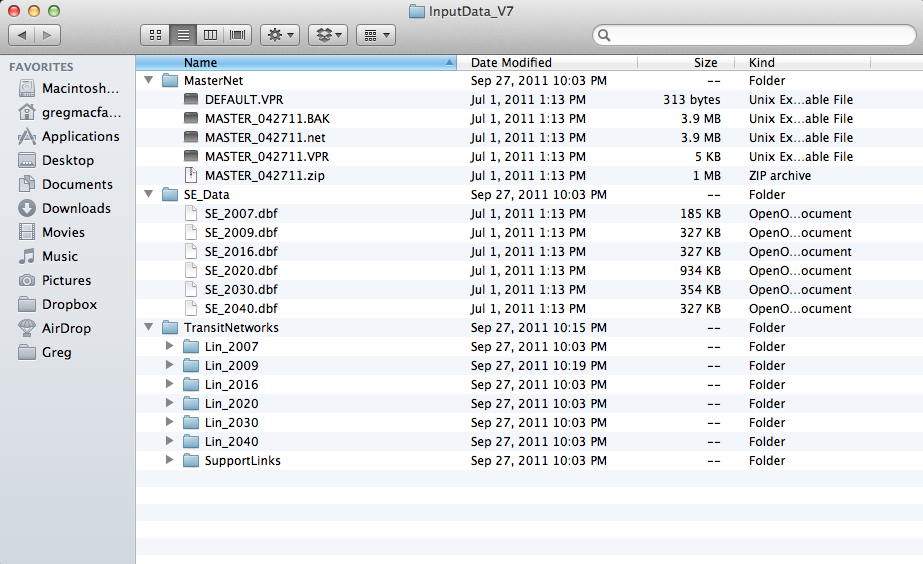
\includegraphics[width = \textwidth]{inputs.png}
	\caption{The Inputs directory, with a view into first-level subfolders.}
	\label{fig:inputsdir}
\end{figure}

The \verb#TransitNetworks/# folder contains subfolders representing the base
transit service plan in the described years. The \verb#Lin_2007/# file,
intuitively, contains the Utah Transit Authority transit network as it existed
in 2007. Within each \verb#Lin_YYYY/# folder are a number of files with the
\verb#YYarea.lin# file name format. These files contain the transit routes in a
given area and year. The naming is typically intuitive (if not consistent), with
\verb#07rail.lin# containing the rail services in 2007. The \verb#X.link# files
hold special links that are used only by transit services and are not part of
the highway network (rail links, for instance). There is also a spreadsheet to
calculate the rail speed given the distance between stations, and a number of
scripts to test if the transit network is complete.\footnote{If there is an
error in your transit network, the model will crash early rather than print
nonsense.} There are also shapefiles of the transit network so that you can
display them in GIS software.



\subsubsection{The Model}
This figure, shown expanded in Figure \ref{fig:modeldir}, contains all the
scripts that comprise the model and is where you will find the model outputs.
As you can see, the directory is clearly labeled with the various model
components numbered in execution order. 

\begin{figure}[tp]
	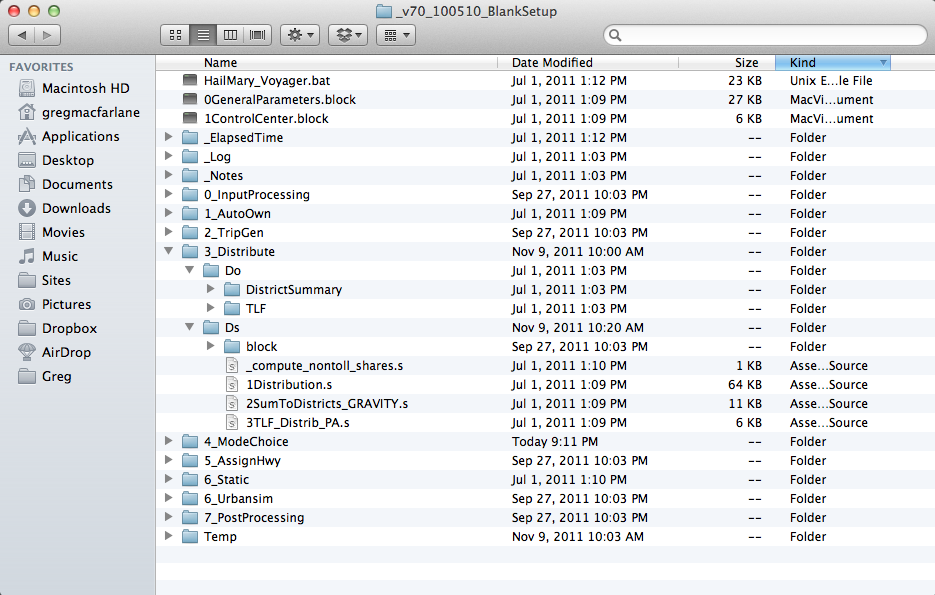
\includegraphics[width = \textwidth]{model.png}
	\caption{The Model directory, with a view into the trip distribution
		model subfolders.}
	\label{fig:modeldir}
\end{figure}


Each model component folder contains two subfolders. As you can see in Figure
\ref{fig:modeldir}, the subfolders for the \verb#3_Dist/# component are
\verb#Do# and \verb#Ds#; these respectively contain the outputs from and the
scripts for the trip distribution models. This naming convention holds through
the directory. The script files in each \verb#Xs# folder are numbered in
execution order, and are given the \verb#.s# file extension. The name of each
file describes what the script does, at least as well as twenty some-odd
characters can.

While I could somewhat exhaustively cover the contents of the inputs directory
in this document, the model directory will essentially be the rest of the
course. But there are three files that need to be explained in detail now.

\paragraph{0GeneralParameters.block}
This is the General Parameters block file, which contains most of the global
variables that are used by the model scripts. The organization of this file is
not ideal, but it's not too bad either. The first 150 lines or so contain path
variables, so the scripts can say \verb#TransitDir# instead of
\verb#../../Inputs/Transit/TransitDirectory/#, for instance. There are also
convenient lists of the aggregation districts and the special generators.

More interesting stuff begins around line 200, where you can set variables for
transit fares, tolls, speed penalties, disutilities, and other stuff. You will
play with some of these numbers throughout the semester, but it's best to leave
them alone if you don't know what you're doing yet.



\paragraph{1ControlCenter.block}
The Control Center block file is something that you will become familiar with
quickly, because this is where you specify which model inputs you want to use
for a given run. You also give your scenario a name (\verb#RID#).  Each time you
run a scenario, you will update the path to the base folder, and change some
input file. There are detailed instructions on how to do this in Section
\ref{sec:modellab}


\paragraph{HailMary\_Voyager.bat}
This is a Windows batch script that issues the proper commands to run the model.
If you double-click on the file, it will open a Windows command prompt and
invite you to start the model. If you right-click on the file, you can instead
open it in a text editor, and see which scripts it calls.

You could run the model by running each of the thirty-or-so scripts in turn, but
the batch file is much easier. Whoever wrote the original HailMary file was
clearly a football fan. If one of your model scripts crashes, you will get a
friendly message saying your star running back has had his leg destroyed by a
300-point lineman (or something similar). If the model runs successfully, you
will get the following triumphant message:
\begin{quote}
\begin{verbatim}
!!!!!!! Touch down!  You win!  All scripts appear to have 
!!!!!!! run correctly! But remember, that's no guarantee 
!!!!!!! that your data is any good. Check the numbers!

!!!!!!! So long, until we meet again on the field of battle!
\end{verbatim}
\end{quote}

If your model crashes, you can make a copy of the \verb#HailMary_Voyager.bat#
file, delete the commands up to where you crashed, and then run the model from
there after you fixed whatever was wrong.


\subsubsection{Model Output}
As the model computes, it will write files into the output folders within the
model directory, and will prefix the output files with the \verb#RID# run name
variable you set in \verb#1ControlCenter.block# This is handy because you can
run two scenarios in the same folder, and you will be able to distinguish the
output files by their \verb#RID#. There are far too many output files to discuss
them in a document of this scope, but I'll introduce some of the most important
ones here.

\paragraph{Log Files} Right in the root directory, the model prints out two log
files, \verb#RID_log.txt# and \verb#RID_log2.txt#. These files give some
high-level statistics on your scenario, such as the fields given in Table
\ref{tab:logs}. On the whole these numbers will not change much between
scenarios in the same year, but a quick look at the numbers can show you if
there were serious problems (like no transit riders). You can also use these
numbers in reports showing things like ``Reducing transit fares by \$0.25
reduces predicted region VMT by 3 percent." \footnote{This is entirely
hypothetical, but would be an interesting analysis for a final project.} 

\begin{table}[t]
	\caption{2009 Base Scenario - Selected Metrics}
	\label{tab:logs}
\begin{center}
\begin{tabular}{l r}
Measurement 			& Value \\ \hline
Total Trips 			& 10,163,525 \\
Total Vehicle Miles Traveled	& 46,363,848 \\
Total Hours of Vehicle Delay	& 74,828 \\
Home-based Work Trips (Motorized)& 1,227,074 \\
All Trips (Non-Motorized) 	& 826,604 \\
All Transit Trips		& 100,109 \\
Average HBW Auto Occupancy 	& 1.171\\
\hline
\end{tabular}
\end{center}
\end{table}

\paragraph{Boardings} Most of my work at the Utah Transit Authority was with
transit riders (obviously). The Boardings files, in
\verb#4_ModeChoice/Mo/Boardings/# show just about everything you want to know
about the transit system. The \verb#RID_2_Route.dbf# file, for instance,
contains the peak and off-peak ridership of all the transit routes, and whether
the riders arrived by car or walk. The \verb#RID_2_OD_Station.dbf# file gives
much of the same information, but broken down by station, so you can look at
which segments of a transit route are under performing. 

This brings up the distinction between PA (Production/Attraction) and OD
(Origin/Destination) numbers. In the model, any trip end at a home is considered
a ``production,'' whether it is the origin or the destination. This is sometimes
confusing, but it simplifies the mathematics substantially: instead of creating
two different home-based work trip matrices for the morning and evening commutes, the
one can just be the transpose of the other. At any rate you will eventually
become familiar with the distinction.

\paragraph{Highway Net} This is perhaps the most important output file of the
travel demand model:
\verb#5_AssignHwy/Ao/UnloadedNetPrefix_4pd.managed.net#. This file
contains the volume by period for every link in the network. I confess that I
don't entirely understand the distinctions between every file in this part of
the model, but you are welcome to explore. One issue- while the transit output
files are visible in Excel, R, etc, the highway outputs require CUBE to
visualize. Sorry.

Now that you know what the model is and how to run it, let's give you some
practice.

\subsection{Lab Exercise}
\label{sec:modellab}
This lab shows you how to run a base year scenario in the Wasatch Front Travel
Model.

\begin{enumerate}
\item{\bf Directory Setup:} Download the three compressed files from the site on
T-Square, and save them to a folder available to you locally. This could be your
local hard disk, an external hard drive, or the space on your Institute account.
When finished, the full model will be approximately 6 GB, so ensure you have the
required space in whatever directory you use.  Unzip the \verb#InputData_V7.zip#
file into this folder.

\item{\bf Folder Setup:} Create a new folder in this directory called
\verb#Base2009/#. Unzip the \verb#BlankModel_090112.zip# file into this subfolder.
You will now have two subfolders in \verb#Base2009/#, \verb#_Inputs# and
\verb#blank_model#. Make a copy of the second folder and change its name to
\verb#Run_mmddyy#, using today's date in the folder name.

\item{\bf Inputs Setup:} Open the \verb#Directory/Base2009/_Inputs/# subfolder.
In a different window, open the \verb#Directory/InputData_V7/# subfolder. Copy
the following files from \verb#InputData_V7# to \verb#Run_mmddyy/_Inputs#:
	\begin{itemize}
	\item{\verb#SE_Data/SE_2009.dbf# $\longrightarrow$ \verb#2_SEData/#}
	\item{\verb#SE_Data/SE_2007.dbf# $\longrightarrow$ \verb#2_SEData/#}
	\item{\verb#MasterNet/MASTER_042711.net# $\longrightarrow$ \verb#3_Highway/#}
	\item{\verb#TransitNetworks/Lin_2009/# $ \longrightarrow$
		\verb#4_Transit/#}
	\end{itemize}

\item{\bf Run Setup:} Open the \verb#1ControlCenter.block# file in a text editor or
in CUBE. Change the following variables to the appropriate values:
	\begin{itemize}
	\item{\verb#UserName = 'Your Name'#}
	\item{\verb#UserCompany = 'Georgia Tech'#}
	\item{\verb#RID = 'Base2009'#}
	\item{\verb#ParentDir = 'Directory\Base2009\Run_mmddyy\'#}
	\item{\verb#DemographicYear = 2009#}
	\item{\verb#SEFile = 'SE_2009.dbf'#}
	\item{\verb#BaseYear = 2009#}
	\item{\verb#SEFileBY = 'SE_2009.dbf'#}
	\item{\verb#NetworkYear = 2009#}
	\item{\verb#pnr_field = PNR09#}
	\item{\verb#LNfield = 'LN09'#}
	\item{\verb#FTfield = 'FT09'#}
	\item{\verb#UnloadedNetPrefix = 'Base2009'#}
	\item{\verb#MLin = 'Lin_2009\'#}
	\item{\verb#IXXIFile = '2009_IXXI.dbf'#}
	\item{\verb#XXFile = '2009_XX.mtx'#}
	\end{itemize}

\item{\bf Hail Mary:}\footnote{Each of the above steps you could do on any
computer. This one will require a computer with CUBE installed.} Double-click on
the \verb#HailMary_Voyager.bat# executable file. A Windows command prompt window
will open, welcoming you to the travel demand model, and inviting you press any
key to continue. I usually press the ``0'' button on the numeric pad because I'm
superstitious, but push whichever key you feel comfortable with. The model will
begin crunching away, and will pretty regularly print output to the command
window.

\item{\bf Wait:} If the model is going to crash, it will usually do so within
the first ten or fifteen minutes. Once you see that the model is into the Trip
Generation scripts, you should be good. Go eat lunch, take a nap, write a blog
post for the ITE website, or all three, and maybe some other things too. A
standard desktop computer will take three to four hours to complete a model run.
When I ran the model professionally, I usually started several model runs when I
left for the evening, and could rely on the outputs being ready when I got to
work the next day.

\end{enumerate}

\paragraph{Assignment Deliverables}
As your deliverable, please complete the information in Table
\ref{tab:modelassign}. Fill in the empty cells, and change the generic file name
to the explicit, complete file name where you obtained your number. Some of the
requested items require some simple arithmetic, but no substantial calculations.
Google Maps may be helpful for identifying locations in Salt Lake City.


\begin{table}[t]
	\caption{2009 Base Scenario - Requested Metrics}
	\label{tab:modelassign}
\begin{center}
\begin{tabular}{l c c}
Measurement 			& Value & Source File\\ \hline
Total lane miles		&	& Log\\
Total freeway VMT		&	& Log\\
Transit share of college trips	&	& Log\\
Work trip share of all trips	&	& Log\\
Daily LRT riders		&	& Boardings\\
Peak CRT riders/revenue mile 	&	& Boardings\\
Daily passengers who walk to route M830 & & Boardings\\
PM volume on I-15 S near 3300 South	&	& Highway Net\\
AM V/C on 500 S near Rice-Eccles Stadium&	& Highway Net\\
\hline
\end{tabular}
\end{center}
\end{table}

\clearpage

\section{TRB Assignment}

Each year at TRB there are a number of presentations on topics relevant to this
course. The purpose of this lab assignment is to acquaint you with this
researchers and those who perform it.

\paragraph{If you are attending TRB}
You should attend a presentation by one of the following researchers (or at
least a paper on which they are a coauthor):
\begin{itemize}
	\item{Chandra Bhat, University of Texas}
	\item{Ram Pendyala, Arizona State University}
	\item{Paul Waddell, University of California - Berkeley}
	\item{Joan Walker, University of California - Berkeley}
	\item{Eric Miller, University of Toronto}
	\item{Stephane Hess, University of Leeds}
	\item{Abolfazl Mohammadian, University of Illinois - Chicago}
	\item{Harry Timmermans, Technische Universiteit Eindhoven}
	\item{Kai Axhausen, Eidgen\"ossische Technische Hochschule (ETH) Z\"urich}
\end{itemize}

You may also attend session 877 or 862, {\em Doctoral Research in Transportation
Modeling}.\footnote{The session is at the Hilton on Thursday morning; I will be
presenting my dissertation defense.}

\paragraph{If you are not attending TRB}
Find a paper published in {\em Transportation Research Record} authored by one
of the researchers listed above.

\paragraph{Deliverable} Write a short but sufficient summary of the research.
Discuss the motivation for the research, the analysis method, and the
conclusions. Also discuss what you learned about travel demand analysis from
this activity.

\clearpage
